% !TeX program = xelatex
% !TeX encoding = UTF-8
\documentclass{article}
\usepackage{ctex}
\usepackage{geometry}
\geometry{a4paper, left=3cm, right=3cm, top=2.5cm, bottom=2.5cm}

\usepackage{graphicx}
\usepackage{enumerate}
\usepackage{amsmath, amssymb, amsthm}
\usepackage{algorithm, algorithmic}
\floatname{algorithm}{算法}
\renewcommand{\algorithmicrequire}{\textbf{Input:}}
\renewcommand{\algorithmicensure}{\textbf{Output:}}

\usepackage{listings}
\usepackage{xcolor}
\usepackage{hyperref}
\hypersetup{colorlinks, citecolor=black, filecolor=black, linkcolor=black, urlcolor=black}

% 代码样式
\lstset{
    language=Python,
    keywordstyle=\color{blue},
    commentstyle=\color{green!50!black},
    stringstyle=\color{red},
    numbers=left,
    numberstyle=\tiny,
    basicstyle=\ttfamily\small,
    frame=single,
    breaklines=true,
    extendedchars=false
}

\title{第三次次上机作业：}
\author{学号：241830137\quad 姓名：朱子健}
\date{\today}

\begin{document}

\maketitle

\section{问题}
考虑函数\(R(x)=\frac{1}{1+x^2}\).利用下列条件做插值逼近，并且与\(R(x)\)的图像比较.
\begin{enumerate}[(1)]
    \item 用节点\(x_i = 5cos(\frac{2i+1}{42}\pi), i = 0, 1,...,20\).\\
          画出20次Lagrange插值多项式的图像；
    \item 用等距节点\(x_i = -5 + i, i = 0, 1,...,10\).\\
          画出10次Newton插值多项式的图像；
    \item 用等距节点\(x_i = -5 + i, i = 0, 1,...,10\).\\
          画出分段线性插值函数的图像；
\end{enumerate}
\section{算法原理与设计}
\subsection{拉格朗日插值法 (Lagrange Interpolation)}
\subsubsection{算法原理}
拉格朗日插值法的核心是通过构造一组基函数 $l_i(x)$ 来形成插值多项式。对于给定 $n+1$ 个互异节点 $(x_i, y_i)$，$i=0,1,\dots,n$，插值多项式 $L_n(x)$ 满足 $L_n(x_i) = y_i$。

\begin{enumerate}
    \item \textbf{拉格朗日基函数}：定义为 $n$ 次多项式，满足在节点 $x_i$ 处为 1，在其他节点处为 0。
    \begin{equation}
    l_i(x) = \prod_{j=0, j \neq i}^{n} \frac{x - x_j}{x_i - x_j} = \frac{(x-x_0)\dots(x-x_{i-1})(x-x_{i+1})\dots(x-x_n)}{(x_i-x_0)\dots(x_i-x_{i-1})(x_i-x_{i+1})\dots(x_i-x_n)}
    \end{equation}
    
    \item \textbf{插值多项式形式}：
    \begin{equation}
    L_n(x) = \sum_{i=0}^{n} y_i l_i(x)
    \end{equation}
\end{enumerate}

\subsubsection{算法设计}
\begin{algorithm}[H]
\caption{计算拉格朗日插值多项式}
\begin{algorithmic}[1]
    \STATE \textbf{输入}: 节点数组 $X = [x_0, \dots, x_n]$, 函数值 $Y = [y_0, \dots, y_n]$, 待计算点 $x$
    \STATE \textbf{输出}: 插值结果 $P$
    \STATE $P \leftarrow 0$
    \FOR{$i = 0$ \TO $n$}
        \STATE $L \leftarrow 1$
        \FOR{$j = 0$ \TO $n$}
            \IF{$j \neq i$}
                \STATE $L \leftarrow L \times \frac{x - x_j}{x_i - x_j}$
            \ENDIF
        \ENDFOR
        \STATE $P \leftarrow P + y_i \times L$
    \ENDFOR
    \RETURN $P$
\end{algorithmic}
\end{algorithm}

\subsection{牛顿插值法 (Newton Interpolation)}

\subsubsection{算法原理}
牛顿插值法利用\textbf{差商 (Divided Difference)} 构造插值多项式。其优点是具有承袭性，即增加一个节点时，只需在原有多项式基础上增加一项。

\begin{enumerate}
    \item \textbf{差商定义}：
    \begin{itemize}
        \item 零阶差商：$f[x_i] = f(x_i)$
        \item 一阶差商：$f[x_i, x_j] = \frac{f(x_j) - f(x_i)}{x_j - x_i}$
        \item $k$ 阶差商：$f[x_0, x_1, \dots, x_k] = \frac{f[x_1, \dots, x_k] - f[x_0, \dots, x_{k-1}]}{x_k - x_0}$
    \end{itemize}
    
    \item \textbf{牛顿插值多项式}：
    \begin{equation}
    N_n(x) = f(x_0) + f[x_0, x_1](x - x_0) + f[x_0, x_1, x_2](x - x_0)(x - x_1) + \dots + f[x_0, \dots, x_n]\omega_n(x)
    \end{equation}
    其中 $\omega_n(x) = \prod_{j=0}^{n-1}(x - x_j)$。
\end{enumerate}

\subsubsection{算法设计}
\begin{algorithm}[H]
\caption{计算牛顿插值多项式}
\begin{algorithmic}[1]
    \STATE \textbf{输入}: 节点 $x_0, \dots, x_n$, 函数值 $f(x_0), \dots, f(x_n)$, 点 $x$
    \STATE \textbf{第一步 (计算差商表)}: 
    \STATE 令 $F_{i,0} = f(x_i)$ （差商表第一列）
    \FOR{$j = 1$ \TO $n$}
        \FOR{$i = j$ \TO $n$}
            \STATE $F_{i,j} \leftarrow \frac{F_{i,j-1} - F_{i-1,j-1}}{x_i - x_{i-j}}$
        \ENDFOR
    \ENDFOR
    \STATE \textbf{第二步 (利用Horner算法求值)}:
    \STATE $y \leftarrow F_{n,n}$
    \FOR{$k = n-1$ \textbf{downto} 0}
        \STATE $y \leftarrow F_{k,k} + (x - x_k) \times y$
    \ENDFOR
    \RETURN $y$
\end{algorithmic}
\end{algorithm}

\subsection{分段线性插值 (Piecewise Linear Interpolation)}

\subsubsection{算法原理}
分段线性插值是在每两个相邻节点 $[x_i, x_{i+1}]$ 之间利用线性函数来逼近原函数。这避免了高次多项式插值可能产生的 Runge 现象。

\begin{enumerate}
    \item \textbf{定义}：在区间 $[a, b]$ 上，设 $a = x_1 < x_2 < \dots < x_{n+1} = b$。在每个子区间 $[x_i, x_{i+1}]$ 上，插值函数 $g_1(x)$ 为线性多项式。
    
    \item \textbf{局部表达式}：当 $x \in [x_i, x_{i+1}]$ 时：
    \begin{equation}
    g_{1,i}(x) = f(x_i) + \frac{f(x_{i+1}) - f(x_i)}{x_{i+1} - x_i}(x - x_i)
    \end{equation}
    
    \item \textbf{误差界}：
    \begin{equation}
    |f(x) - g_1(x)| \le \frac{h^2}{8} \max |f''(x)|, \quad h = \max(x_{i+1} - x_i)
    \end{equation}
\end{enumerate}

\subsubsection{算法设计}
\begin{algorithm}[H]
\caption{计算分段线性插值函数}
\begin{algorithmic}[1]
    \STATE \textbf{输入}: 已排序节点数组 $X$, 函数值数组 $Y$, 待求点 $x$
    \STATE \textbf{第一步 (定位区间)}: 
    \STATE 在 $X$ 中查找 $i$，使得 $x_i \le x \le x_{i+1}$ （可使用二分查找）
    \STATE \textbf{第二步 (线性计算)}:
    \STATE $k \leftarrow \frac{y_{i+1} - y_i}{x_{i+1} - x_i}$
    \STATE $y \leftarrow y_i + k \times (x - x_i)$
    \RETURN $y$
\end{algorithmic}
\end{algorithm}

\section{结果分析}
根据题目给定的节点和原函数 $R(x)=\frac{1}{1+x^2}$，我们可以写出这三种插值函数的具体数学表达式。
\subsection{20 次 Lagrange 插值多项式}
所用节点为：
\[ x_i = 5\cos\left(\frac{2i+1}{42}\pi\right), \quad i = 0, 1, \dots, 20 \]
对应的函数值为 $y_i = \frac{1}{1+x_i^2}$。则具体的 20 次拉格朗日插值多项式表达式为：
\begin{equation}
L_{20}(x) = \sum_{i=0}^{20} \left( \frac{1}{1 + 25\cos^2\left(\frac{2i+1}{42}\pi\right)} \cdot \prod_{\substack{j=0 \\ j \neq i}}^{20} \frac{x - 5\cos\left(\frac{2j+1}{42}\pi\right)}{5\cos\left(\frac{2i+1}{42}\pi\right) - 5\cos\left(\frac{2j+1}{42}\pi\right)} \right)
\end{equation}

\subsection{10 次 Newton 插值多项式}
所用等距节点为 $\{-5, -4, -3, -2, -1, 0, 1, 2, 3, 4, 5\}$。
10次牛顿插值多项式的具体展开式为：
\begin{equation}
\begin{aligned}
N_{10}(x) &= c_0 + c_1(x+5) + c_2(x+5)(x+4) + c_3(x+5)(x+4)(x+3) \\
&\quad + c_4(x+5)(x+4)(x+3)(x+2) + \dots \\
&\quad + c_{10}(x+5)(x+4)(x+3)(x+2)(x+1)x(x-1)(x-2)(x-3)(x-4)
\end{aligned}
\end{equation}
其中，各项差商系数 $c_k = f[x_0, x_1, \dots, x_k]$ 经计算（保留五位有效小数）如下：
\[
\begin{array}{llll}
c_0 \approx 0.03846 & c_1 \approx 0.02036 & c_2 \approx 0.01041 & c_3 \approx 0.00633 \\
c_4 \approx 0.00430 & c_5 \approx -0.00204 & c_6 \approx -0.00113 & c_7 \approx 0.00109 \\
c_8 \approx -0.00043 & c_9 \approx 0.00011 & c_{10} \approx -0.00002 & 
\end{array}
\]

\subsection{分段线性插值多项式}
等距节点同样为 $x_i \in \{-5, -4, \dots, 5\}$，函数值 $y_i \in \{\frac{1}{26}, \frac{1}{17}, \frac{1}{10}, \frac{1}{5}, \frac{1}{2}, 1, \dots\}$。通过计算两点间的斜率，我们可以写出精确的 10 段线性函数表达式：
\begin{equation}
P(x) = \begin{cases}
\frac{1}{26} + \frac{9}{442}(x+5), & x \in [-5, -4] \\
\frac{1}{17} + \frac{7}{170}(x+4), & x \in [-4, -3] \\
\frac{1}{10} + \frac{1}{10}(x+3), & x \in [-3, -2] \\
\frac{1}{5} + \frac{3}{10}(x+2), & x \in [-2, -1] \\
\frac{1}{2} + \frac{1}{2}(x+1), & x \in [-1, 0] \\
1 - \frac{1}{2}x, & x \in [0, 1] \\
\frac{1}{2} - \frac{3}{10}(x-1), & x \in [1, 2] \\
\frac{1}{5} - \frac{1}{10}(x-2), & x \in [2, 3] \\
\frac{1}{10} - \frac{7}{170}(x-3), & x \in [3, 4] \\
\frac{1}{17} - \frac{9}{442}(x-4), & x \in [4, 5]
\end{cases}
\end{equation}

\subsection{图像对比}
通过编写 Python 程序计算并绘制插值曲线，我们可以得出如下分析结论：
\begin{figure}[htbp]
    \centering
    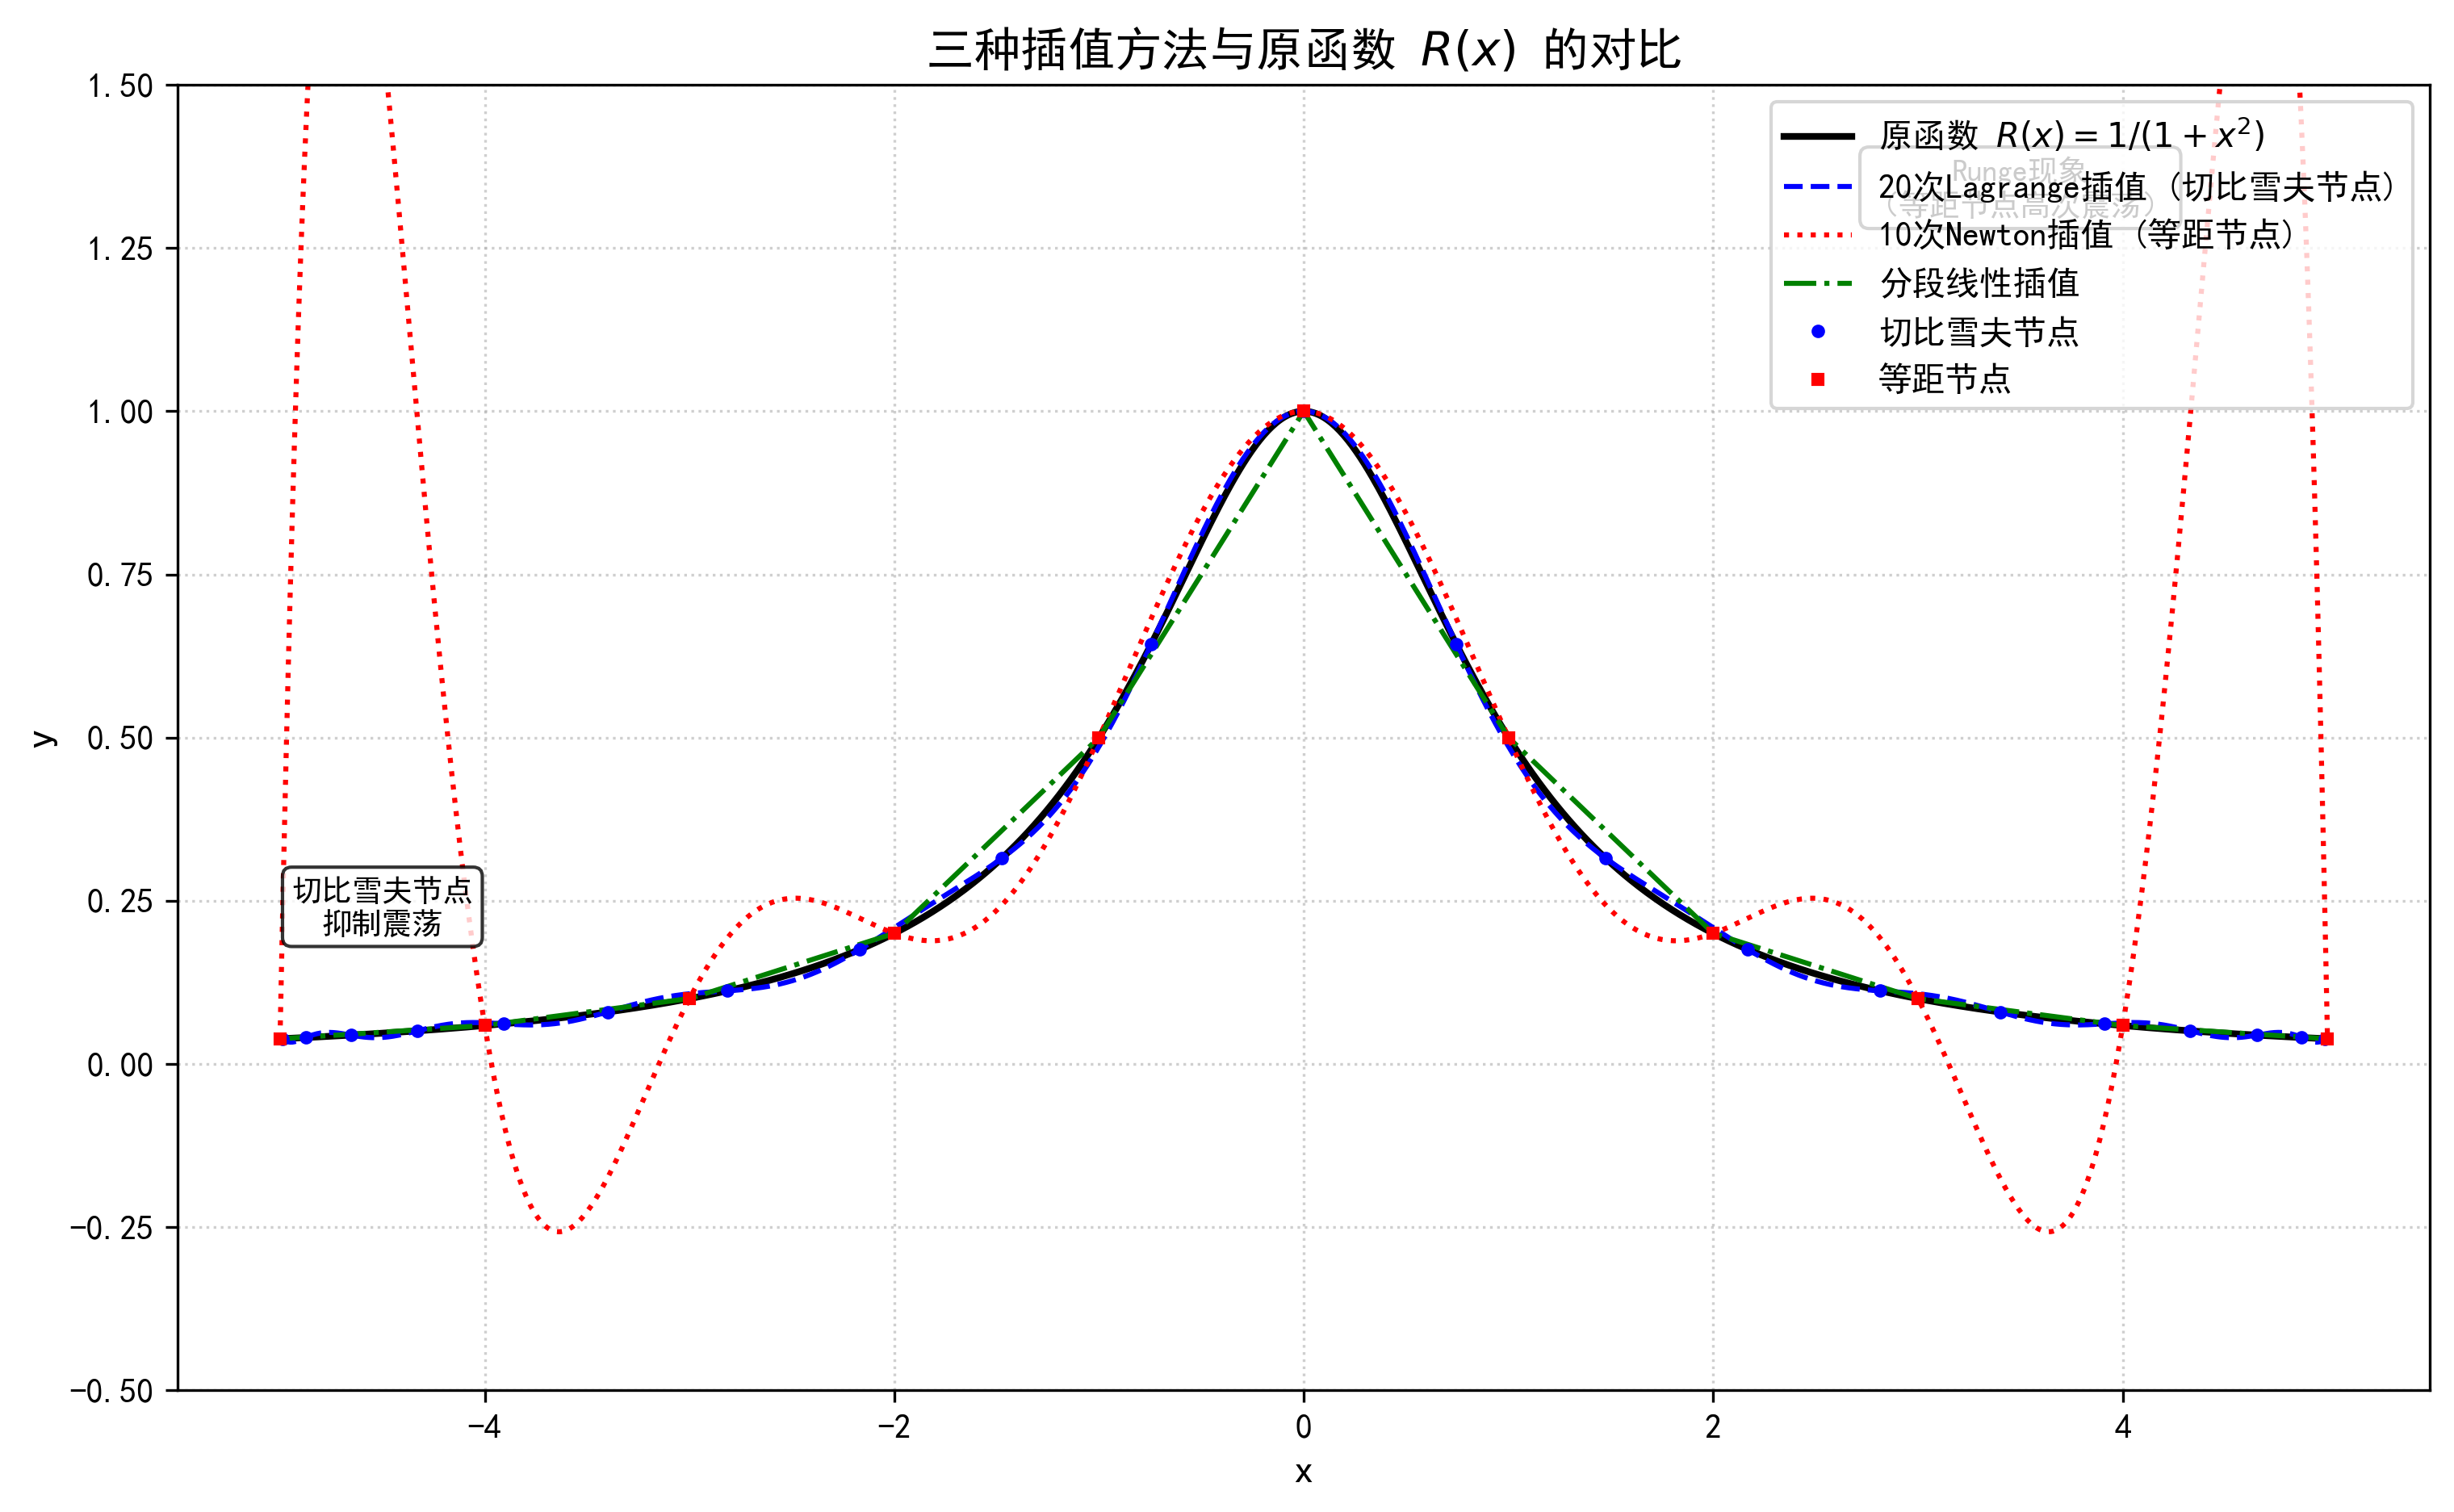
\includegraphics[width=0.8\textwidth]{plot_results.png} 
    \caption{三种插值方法与原函数 $R(x)$ 的对比示意图}
    \label{fig:plots}
\end{figure}
\begin{enumerate}
    \item \textbf{Runge 现象（等距节点高次插值）}：
    观察10次牛顿插值多项式的图像，在区间中心（0附近）逼近效果较好，但在区间边缘（$[-5, -3]$ 和 $[3, 5]$）出现了极其剧烈的震荡。这正是经典的 \textbf{Runge 现象}，说明对于 $R(x)=\frac{1}{1+x^2}$ 这样的函数，盲目增加等距节点的插值多项式次数，不仅无法提高精度，反而会导致边界处的误差发散。
    
    \item \textbf{切比雪夫节点的优化效果}：
    在第(1)题中，使用了 20 次拉格朗日插值，但节点选取了切比雪夫零点（即两端密、中间疏的节点分布）。图像显示，尽管次数高达20次，不仅没有出现 Runge 现象，反而极其精确地贴合了原函数曲线。这验证了改变节点分布是克服 Runge 现象的有效手段。
    
    \item \textbf{分段线性插值的稳健性}：
    第(3)题的分段线性插值在整个区间内表现出高度的稳定性。虽然它在节点处的导数不连续（表现为折线），逼近精度受限于节点数量，但它将误差严格限制在局部子区间内，完全避免了全局多项式的剧烈波动。
\end{enumerate}

\newpage
\section{附录：Python源代码实现}
本代码同时实现了 Lagrange、Newton 和分段线性插值，并将计算结果输出为数据以便于画图比对。

\begin{lstlisting}[language=Python]
import math
import matplotlib.pyplot as plt
import numpy as np

# 设置 matplotlib 支持中文显示
plt.rcParams['font.sans-serif'] = ['SimHei']   # 用于正常显示中文标签
plt.rcParams['axes.unicode_minus'] = False    # 解决负号显示问题

# ---------- 插值算法实现（与之前相同） ----------
def R(x):
    """原函数 R(x) = 1/(1+x^2)"""
    return 1.0 / (1.0 + x * x)

def lagrange(x, xi, yi):
    """拉格朗日插值"""
    n = len(xi)
    result = 0.0
    for i in range(n):
        term = yi[i]
        for j in range(n):
            if i != j:
                term *= (x - xi[j]) / (xi[i] - xi[j])
        result += term
    return result

def newton(x, xi, yi):
    """牛顿插值（差商表 + Horner）"""
    n = len(xi)
    f = [[0.0] * n for _ in range(n)]
    for i in range(n):
        f[i][0] = yi[i]
    for j in range(1, n):
        for i in range(j, n):
            f[i][j] = (f[i][j-1] - f[i-1][j-1]) / (xi[i] - xi[i-j])
    res = f[n-1][n-1]
    for i in range(n-2, -1, -1):
        res = f[i][i] + (x - xi[i]) * res
    return res

def piecewise_linear(x, xi, yi):
    """分段线性插值"""
    n = len(xi)
    if x <= xi[0]:
        return yi[0]
    if x >= xi[-1]:
        return yi[-1]
    for i in range(n-1):
        if xi[i] <= x <= xi[i+1]:
            return yi[i] + (yi[i+1] - yi[i]) * (x - xi[i]) / (xi[i+1] - xi[i])
    return 0.0

# ---------- 生成节点 ----------
# 1. 切比雪夫节点（用于20次Lagrange插值）
PI = math.acos(-1.0)
x_cheb = [5.0 * math.cos((2.0*i + 1.0) / 42.0 * PI) for i in range(21)]
y_cheb = [R(x) for x in x_cheb]

# 2. 等距节点（用于Newton和分段线性插值）
x_eq = [-5.0 + i for i in range(11)]
y_eq = [R(x) for x in x_eq]

# ---------- 生成绘图数据 ----------
x_plot = np.linspace(-5, 5, 1000)          # 1000个点用于平滑绘图
y_true = R(x_plot)
y_lagrange = [lagrange(x, x_cheb, y_cheb) for x in x_plot]
y_newton = [newton(x, x_eq, y_eq) for x in x_plot]
y_piecewise = [piecewise_linear(x, x_eq, y_eq) for x in x_plot]

# ---------- 绘图 ----------
plt.figure(figsize=(12, 7))

# 原函数
plt.plot(x_plot, y_true, 'k-', linewidth=2, label='原函数 $R(x)=1/(1+x^2)$')

# 20次Lagrange插值（切比雪夫节点）
plt.plot(x_plot, y_lagrange, 'b--', linewidth=1.5, label='20次Lagrange插值 (切比雪夫节点)')

# 10次Newton插值（等距节点，Runge现象）
plt.plot(x_plot, y_newton, 'r:', linewidth=1.5, label='10次Newton插值 (等距节点)')

# 分段线性插值
plt.plot(x_plot, y_piecewise, 'g-.', linewidth=1.5, label='分段线性插值')

# 标记节点（可选，增强可读性）
plt.plot(x_cheb, y_cheb, 'bo', markersize=3, label='切比雪夫节点')
plt.plot(x_eq, y_eq, 'rs', markersize=3, label='等距节点')

# 设置坐标轴范围（突出Runge现象，同时保证其他曲线可见）
plt.xlim(-5.5, 5.5)
plt.ylim(-0.5, 1.5)          # 牛顿插值在边界处会剧烈震荡，限制y轴范围以观察全貌

plt.xlabel('x', fontsize=12)
plt.ylabel('y', fontsize=12)
plt.title('三种插值方法与原函数 $R(x)$ 的对比', fontsize=14)
plt.legend(loc='upper right', fontsize=10)
plt.grid(True, linestyle=':', alpha=0.6)

# 添加文字说明Runge现象和切比雪夫节点效果
plt.text(3.5, 1.3, 'Runge现象\n（等距节点高次震荡）', ha='center', fontsize=9,
         bbox=dict(boxstyle="round,pad=0.3", facecolor="white", alpha=0.8))
plt.text(-4.5, 0.2, '切比雪夫节点\n抑制震荡', ha='center', fontsize=9,
         bbox=dict(boxstyle="round,pad=0.3", facecolor="white", alpha=0.8))

# 保存图像（与LaTeX文档中引用的文件名一致）
plt.savefig('plot_results.png', dpi=300, bbox_inches='tight')
plt.show()

print("图像已保存为 plot_results.png")
\end{lstlisting}
\end{document}